\documentclass{article}
% Change "article" to "report" to get rid of page number on title page
\usepackage{amsmath,amsfonts,amsthm,amssymb}
\usepackage{setspace}
\usepackage{Tabbing}
\usepackage{fancyhdr}
\usepackage{lastpage}
\usepackage{extramarks}
\usepackage{chngpage}
\usepackage{soul,color}
\usepackage{graphicx,float,wrapfig}
\usepackage{multirow}
\usepackage{enumerate}
\usepackage{comment} 
% In case you need to adjust margins:
\topmargin=-0.45in      %
\evensidemargin=0in     %
\oddsidemargin=0in      %
\textwidth=6.5in        %
\textheight=9.0in       %
\headsep=0.25in         %

% Homework Specific Information
\newcommand{\hmwkTitle}{Biased Bar Test}
\newcommand{\hmwkClass}{}
\newcommand{\hmwkAuthorName}{Donglai\ Wei}


% Setup the header and footer
\pagestyle{fancy}                                                       %
\lhead{\hmwkAuthorName}                                                 %
\rhead{\firstxmark}                                                     %
\lfoot{\lastxmark}                                                      %
\cfoot{}                                                                %
\rfoot{Page\ \thepage\ of\ \pageref{LastPage}}                          %
\renewcommand\headrulewidth{0.4pt}                                      %
\renewcommand\footrulewidth{0.4pt}                                      %

% This is used to trace down (pin point) problems
% in latexing a document:
%\tracingall

%%%%%%%%%%%%%%%%%%%%%%%%%%%%%%%%%%%%%%%%%%%%%%%%%%%%%%%%\begin{enumerate}

% Some tools
\newcommand{\enterProblemHeader}[1]{\nobreak\extramarks{#1}{#1 continued on next page\ldots}\nobreak%
                                    \nobreak\extramarks{#1 (continued)}{#1 continued on next page\ldots}\nobreak}%
\newcommand{\exitProblemHeader}[1]{\nobreak\extramarks{#1 (continued)}{#1 continued on next page\ldots}\nobreak%
                                   \nobreak\extramarks{#1}{}\nobreak}%

\newlength{\labelLength}
\newcommand{\labelAnswer}[2]
  {\settowidth{\labelLength}{#1}%
   \addtolength{\labelLength}{0.25in}%
   \changetext{}{-\labelLength}{}{}{}%
   \noindent\fbox{\begin{minipage}[c]{\columnwidth}#2\end{minipage}}%
   \marginpar{\fbox{#1}}%

   % We put the blank space above in order to make sure this
   % \marginpar gets correctly placed.
   \changetext{}{+\labelLength}{}{}{}}%

\setcounter{secnumdepth}{0}
\newcommand{\homeworkProblemName}{}%
\newcounter{homeworkProblemCounter}%
\newenvironment{homeworkProblem}[1][Problem \arabic{homeworkProblemCounter}]%
  {\stepcounter{homeworkProblemCounter}%
   \renewcommand{\homeworkProblemName}{#1}%
   \section{\homeworkProblemName}%
   \enterProblemHeader{\homeworkProblemName}}%
  {\exitProblemHeader{\homeworkProblemName}}%

\newcommand{\problemAnswer}[1]
  {\noindent\fbox{\begin{minipage}[c]{\columnwidth}#1\end{minipage}}}%

\newcommand{\problemLAnswer}[1]
  {\labelAnswer{\homeworkProblemName}{#1}}

\newcommand{\homeworkSectionName}{}%
\newlength{\homeworkSectionLabelLength}{}%
\newenvironment{homeworkSection}[1]%
  {% We put this space here to make sure we're not connected to the above.
   % Otherwise the changetext can do funny things to the other margin

   \renewcommand{\homeworkSectionName}{#1}%
   \settowidth{\homeworkSectionLabelLength}{\homeworkSectionName}%
   \addtolength{\homeworkSectionLabelLength}{0.25in}%
   \changetext{}{-\homeworkSectionLabelLength}{}{}{}%
   \subsection{\homeworkSectionName}%
   \enterProblemHeader{\homeworkProblemName\ [\homeworkSectionName]}}%
  {\enterProblemHeader{\homeworkProblemName}%

   % We put the blank space above in order to make sure this margin
   % change doesn't happen too soon (else \sectionAnswer's can
   % get ugly about their \marginpar placement.
   \changetext{}{+\homeworkSectionLabelLength}{}{}{}}%

\newcommand{\sectionAnswer}[1]
  {% We put this space here to make sure we're disconnected from the previous
   % passage

   \noindent\fbox{\begin{minipage}[c]{\columnwidth}#1\end{minipage}}%
   \enterProblemHeader{\homeworkProblemName}\exitProblemHeader{\homeworkProblemName}%
   \marginpar{\fbox{\homeworkSectionName}}%

   % We put the blank space above in order to make sure this
   % \marginpar gets correctly placed.
   }%

%%%%%%%%%%%%%%%%%%%%%%%%%%%%%%%%%%%%%%%%%%%%%%%%%%%%%%%%%%%%%



%%%%%%%%%%%%%%%%%%%%%%%%%%%%%%%%%%%%%%%%%%%%%%%%%%%%%%%%%%%%%
% Make title
\title{\vspace{0.3in}\textmd{\textbf{\hmwkTitle}}}
\date{2010.8.3}
\author{\textbf{\hmwkAuthorName}}
%%%%%%%%%%%%%%%%%%%%%%%%%%%%%%%%%%%%%%%%%%%%%%%%%%%%%%%%%%%%%

\begin{document}
\begin{spacing}{1.1}
\maketitle

\section{0)Set Up:}
{\bf Set Up:}\\
1)40/200 Restaurants,each has 50 customers.\\ \\
2)5 by 5 words,10 real bars with frequency weight:[1,2,1,3,1,10,8,1,6,4]\\ 
(the first 5 are vertical bars and the last 5 are horizontal,the most frequent bars are the top 2 horizontal bars)\\\\
3)Hyperparameter:$\alpha=1$,$\gamma=1.5$,$\lambda_{0}=0.2$\\ \\
4)Annealing Scheme(anneal all search function): Temperature $T\in[0.2,0.4,0.6,0.8,1]^{(0.5)}$\\ 

\section{1)40 Restaurants:}
1) (Figure 1, left)Basically, our ME search finds most of the bars.\\ \\
2) Since the number of Restaurants is small, some bars may not happen frequently. Thus a better explanation of the data maybe of less than 10 bars.\\ \\
3) The last 5 noisy dishes are all made of 1 or 2 tables with small number of customers compared to the first 7. Since the evidence of some vertical bars are not
sufficient, it is better to leave them noisy.\\ \\
4) Figure 1(right) is one more run after Figure 1(left) with T=$0.2^{0.5}\sim$(0.44), which gets rid of noisy dishes but has worse log Probability.
\begin{figure}
 \centering
   \begin{tabular}{cc}    
     \resizebox{40mm}{!}{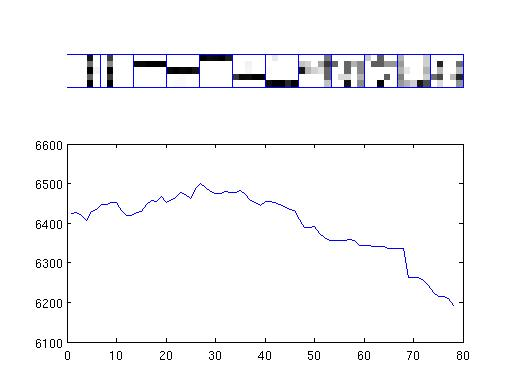
\includegraphics{bias_05_4.jpg}} &
     \resizebox{40mm}{!}{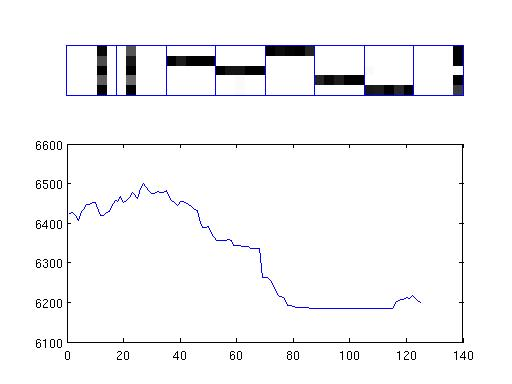
\includegraphics{bias_05_bar.jpg}}\\ 
        \end{tabular}
    \caption{left: after 5 iterations; right: 9 nice bars has worse log Probability}
    \label{fig:by:table} 
\end{figure}

\newpage
\section{2)200 Restaurants:}
1) (Figure 2) With more Restaurants, our ME search finds all of the bars.\\ \\
2) Since the number of Restaurants is small, some bars may not happen frequently. Thus a better explanation of the data maybe of less than 10 bars.\\ \\
3) Something weird is that the fourth dish and the second to last dish refuse to be merged...\\
Merging these two dishes won't change t-term and the $\lambda_{0}$ and $\gamma$ are not strong enough to force them to merge.\\ \\
4) The second dish is noisy and can be eliminated by decompose dish with T$\sim$0.5. It means the annealing process can be improve\\
\begin{figure}
 \centering
 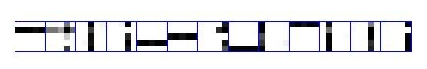
\includegraphics{200_bias_05_bar.jpg}
 caption{200 restaurants, after 5 iterations}   
\end{figure}

\end{spacing}
\end{document}

%%%%%%%%%%%%%%%%%%%%%%%%%%%%%%%%%%%%%%%%%%%%%%%%%%%%%%%%%%%%%
